\documentclass[../main.text]{report}
\begin{document}
\subsection{Seconde conjecture}
\subsubsection{Introduction}

La conjecture que nous allons tester ici est la suivante: 

	\begin{Conj}
	Pour tout $n = 6, 7, ...$, il existe un nombre premier $p$ tel que $6n-p$ et $6n+p$ sont tous les deux premiers. \footnote{Conjecture 2.3 de maths.nju.edu.cn/\~zwsun/}
	\end{Conj}
	

Nous allons d'abord vérifier que cette conjecture tient pour les nombres premiers, puis vérifier si celle-ci tient aussi pour les ensembles aléatoires suivant leur distribution.
La procédure pour analyser cette conjecture est donc la suivante: pour chaque $n\in \mathbb{N}, 6 \leq n \leq 10000$, nous vérifierons pour chaque $p \in R_k$ si $(6n-p,6n+p) \in R_k^2$. Nous collecterons alors tout $n$ tel que $\neg P(n)$ dans des tableaux de données\footnote{le code pour ces tableaux de donnés est donné dans l'appendice \ref{code:conj_2_3_report}. Ceux-ci sont sauvegardés dans le dossier /data/conjecture\_2\_3/ du github} afin d'analyser, pour chaque ensemble ou chaque groupe d'ensemble, le nombre et la distribution des erreurs.

\subsubsection{Analyse}


%Utilisons les notations $R_{k_n}$, $U_{k_n}$ pour désigner les ensembles $\{i \in R_k ~|~i < n \}$ (respectivement, $\{i \in R_k ~|~i < n \}$).
Soit $P(n)$ l'assertion "pour un certain $n \in \mathbb{N}, n\geq6$, Il existe $p \in R_{k}, p \leq n$ tel que $6n-p \in R_k$ et $6n+p \in R_k$".

En utilisant un algorithme \footnote{voir appendice: \ref{code:Error_mapping} - "py\_code/test\_conj\_2\_3.py" }, nous avons pu observer que, pour les nombres premiers, l'assertion est vraie pour tout $6 < n \leq 10^6$ .
Le même algorithme confirme que la conjecture n'est pas vérifiée, du moins pour tout $n \geq 6$, en ce qui concerne les ensembles aléatoires. Cependant, il semble que certains de ces ensembles possèdent des propriétés similaires si l'on choisit un $n$ plus grand.

Nous nous intéressons au nombre d'erreurs (c'est à dire le nombre d'entiers $n$ pour lesquelle l'assertion n'est pas vérifiée), ainsi que le plus grand entier pour lequel l'assertion est fausse. Cette dernière information est intéressante car si ce plus grand entier est petit, alors la conjecture est vérifiée pour tout $n$ plus grand.

Le graphique \ref{fig:failures_2_3} ci-dessous représente en abscisses le nombre total d'erreur (c'est à dire $\#\{n | \neg P(n)\}$) pour $n \in \{6,...,10^5\}$, et en ordonnés le plus grand entier pour lequel l'assertion est fausse (ou bien $\max \{n | \neg P(n)\}$). Chaque point représente un ensemble. Les ensembles ayant les meilleurs "performances" sont alors situés en bas à gauche: ceux-ci ont alors un faible nombre d'erreurs, et vérifie l'assertion pour tout $n$ plus grand. 

\begin{figure}[H]
\centering
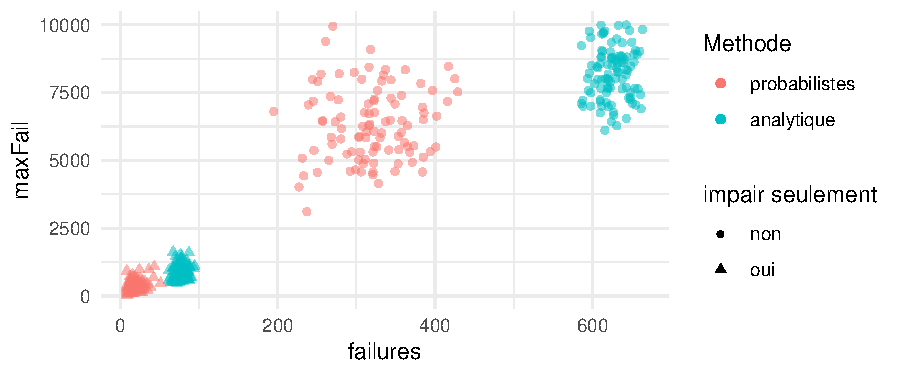
\includegraphics{plot_failure_maxfaile_c_2_3}
\caption{}
\label{fig:failures_2_3}
\end{figure}

Nous débuterons par remarquer que l'existence d'un entier $p$ répondant aux critères de la conjecture n'est pas rare. En effet, pour $ n \in \{6,...,10000\}$, l'assertion est vérifiée par près de 99\% des entiers $n$ testés pour chaque ensemble (moins de 650 erreurs). 

Les ensembles non restreints aux nombres impairs génèrent tout de même un nombre assez élevé d'erreurs: plus de 200 erreurs pour la quasi-totalité de ces ensembles.
De plus, ces erreurs persistent assez tardivement: pour la majorité de ces ensembles, il existe (au moins) un entier $n > 5000$ pour lequel l'assertion est fausse. 


Les ensembles composés de nombres impairs ont cependant de bien meilleurs performances . Ceux-ci ont un faible nombre d'erreurs (moins de 50 pour les ensembles générés par l'algorithme probabiliste, moins de 100 pour les ensembles générés par les algorithmes analytiques, voir figure \ref{fig:boxplots_Odd}). 
De plus, le plus grand entier pour lequel l'assertion n'est pas vérifiée est relativement faible: cela signifie que pour tout entier $n > 1500$, l'assertion est vérifiée. Pour plus de trois quarts des ensembles aléatoires générés par l'algorithme probabiliste, on a même l'assertion vérifiée pour tout $n > 500$.
Finalement, on remarque aussi que les ensembles crées par l'algorithme probabiliste ont des performances sensiblement meilleures. Cela est surement du au fait qu'ils possèdent sensiblement plus d'éléments que les autre ensembles (voir figure \ref{fig:comparison_all_random_sets}), ou alors parce que leur distribution est plus proche de celles des nombres premiers.

Les diagrammes en boites \ref{fig:boxplots} et \ref{fig:boxplots_Odd} ci-dessus offrent un aperçu de la distribution des erreurs. La seconde figure se concentre sur les ensembles impairs afin de faciliter la lecture du graphique.

\begin{figure}[H]
\centering
	\subfigure[Plus grand n ne vérifiant pas l'assertion]{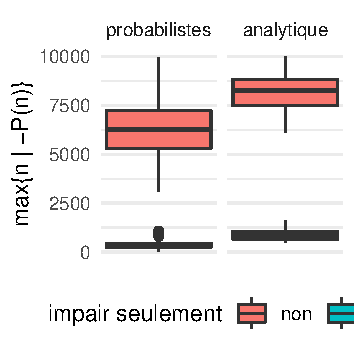
\includegraphics{C23_MaxFail_BoxPlot}}%
	\subfigure[Nombre d'erreurs]{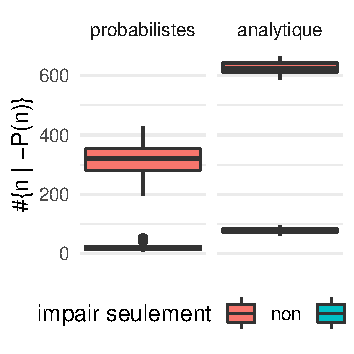
\includegraphics{C23_FailCount_BoxPlot}}
	\caption{Diagrammes en boite}
	\label{fig:boxplots}
\end{figure}

\begin{figure}[H]
\centering
	\subfigure[Plus grand n ne vérifiant pas l'assertion]{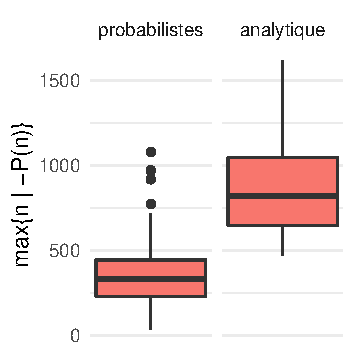
\includegraphics{C23_MaxFail_BoxPlot_Odd}}%
	\subfigure[Nombre d'erreurs]{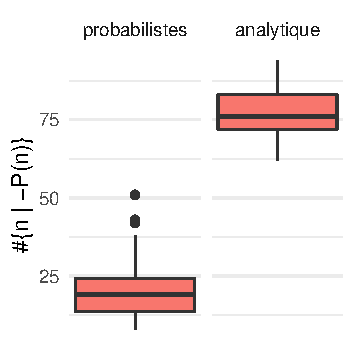
\includegraphics{C23_FailCount_BoxPlot_Odd}}
	\caption{Diagrammes en boite - ensembles impairs.}
	\label{fig:boxplots_Odd}
\end{figure}

Il existe trois ensembles vérifiant l'assertion pour tout $n, 100 \leq n \leq 10000$:
\begin{itemize}
	\item l'ensemble probabiliste impair 032 vérifiant l'assertion pour tout $n > 38$
	\item l'ensemble probabiliste impair 091 vérifiant l'assertion pour tout $n > 74$
	\item l'ensemble probabiliste impair 033 vérifiant l'assertion pour tout $n > 97$
\end{itemize}
Pour ces ensembles, l'assertion tient, comme pour les nombres premiers, au moins jusqu'à $n=10^6$.  

De plus, au delà de 100, il existe 50 ensembles ayant moins de 5 erreurs. 
Il apparait alors que la probabilité d'une erreur diminue, et tend vers 0, lorsque n devient grand, comme le fait remarquer le graphique ci-dessous, représentant le nombre moyen d'erreurs sur un intervalle $[6+10n, 6+11n[$.
\begin{figure}[H]
\centering
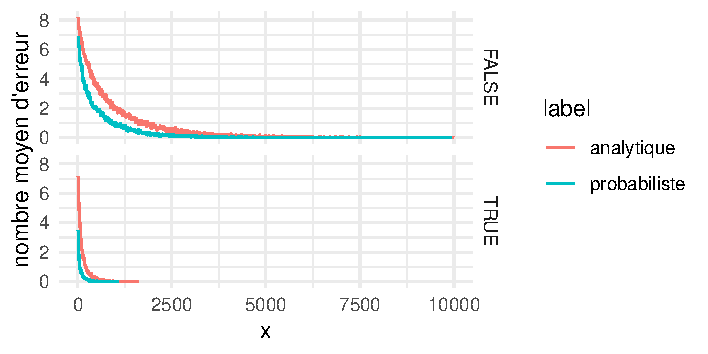
\includegraphics{conjecture_2_3_10k_bin5_line}
\caption{Diagramme représentant le nombre moyen d'erreur sur l'intervale $]6+10n, 6+11n]$}
\label{fig:conjecture_2_3_10k_bin5_line}
\end{figure}

On observe ici que pour les ensembles aléatoires impairs, le nombre moyen d'erreurs tend très rapidement vers 0 jusqu'à qu'aucune erreur n'apparaisse aux alentours de 1200. Cette même statistique diminue moins vite pour les autres ensembles, mais tend elle aussi vers 0.
Il semble alors que pour un $n$ suffisement grand, la probabilité que l'assertion soit fausse diminue, voire devient négligeable pour les ensembles impairs. 

\subsubsection{Conclusion de l'analyse}
Certains ensembles aléatoires, notemment les ensembles impairs, semblent vérifier la conjecture pour $n$ plus grand que 6. Pour certains d'entre eux, il semble qu'il existe un entier $m \in \mathbb{N}$ à partir duquel, pour tout $n > m$, il existe toujours un élement $p < n$ dans l'ensemble tel que $p, 6n-p$ et $6n+p$ sont tous dans l'ensemble. Nous nous demandons alors si cette conjecture tient pour les nombres premiers, comme pour certains ensembles aléatoires démontrant de bonnes "performances", qu'à cause d'une distribution "heureuse" au départ, lorsque $n$ est suffisement petit. Lorsque $n$ est suffisement grand, la probabilité d'une erreur est alors si faible qu'elle devient négligeable.  


%\begin{figure}[h]
%\centering
%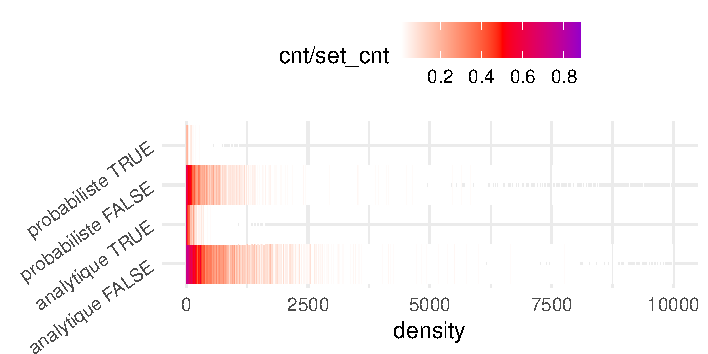
\includegraphics{heat_conjecture_2_3}
%\caption{diagramme représentant le nombre moyen d'erreur (entier ne vérifiant pas la conjecture) sur l'interval $(n,n+5]$}
%\label{fig:heat_conjecture_2_3		}
%\end{figure}

%Cela semble avoir du sens dans la mesure où le nombres d'elements $p$ continue d'augmenter lorsque p augmente, 



\end{document}
